\section{Oracle Lower Bounds}
\subsection{Review : Rates of Convergence}
\begin{frame}{Review : Rates of Convergence}
    \setstretch{1.3}
    \textbf{Subgradient method}
    \begin{itemize}
        \item  $x_{t+1} = x_t- \eta g_t$, where $g_t \in \partial f(x_t)$
    \end{itemize}
    
    \textbf{Gradient method}
    \begin{itemize}
        \item  $x_{t+1} = x_t- {\eta}{\nabla}f(x_t)$
    \end{itemize}
    
    \textbf{Subgradient method for Lipschitz convex functions}
    \begin{itemize}
        \item  Convergence rate: $ \mathcal{O}\left({1 \over {\sqrt{T}}}\right)  \leftrightarrow $ for error $ \epsilon$, $\mathcal{O}\left({1 \over \epsilon^2}\right)$
    \end{itemize}
    
    \textbf{Gradient descent for smooth convex functions}
    \begin{itemize}
        \item  Convergence rate: $ \mathcal{O}\left({1 \over T}\right)  \leftrightarrow $ for error $ \epsilon$, $ \mathcal{O}\left({1 \over \epsilon}\right)$
    \end{itemize}

    \textbf{Gradient descent for $\beta$-smooth and $\alpha$-strongly convex functions}
    \begin{itemize}
        \item  Convergence rate: where $ \kappa = {\beta \over \alpha}$ , $ \mathcal{O}\left(\left({\kappa-1 \over \kappa+1}\right)^T\right)  \leftrightarrow $ for error $ \epsilon$, $ \mathcal{O}\left(\kappa{\log\left({1 \over \epsilon}\right)}\right)$
    \end{itemize}
    
\end{frame}



\subsection{Oracle model of computation}
\begin{frame}{Oracle model of computation}
    \setstretch{1.3}
    \textbf{What do we know about our function?}
    \begin{spacing}{0.9}
    $$\min:f(x), s.t: x \in \mathfrak{X}=\mathds{R}^d$$
    \end{spacing}
    
    \begin{itemize}
        \item The way to make precise the idea of complexity in terms of how of convergence rate is to say what do we use for every single algorithm.
        \item In other words, think about this as though we don't actually know our function $f$ at all. All we have access to is something that I'll call an Oracle. 
        
    \end{itemize}
    $$x\longrightarrow\fbox{First order Oracle}\longrightarrow f(x),{\nabla}f(x) {\text{ or }} g_x {\in} {\partial}f(x)$$

    \begin{itemize}
        \item Suppose the only access to our function $f$ is through this first-order oracle.
        \item Then we can frame the question as follows. How many calls to the Oracle do we need \textbf{in the worst case} over a class of functions, in order to guarantee error $\epsilon$?
    \end{itemize}
\end{frame}
% 첫번째 문장을 더 짧게
\begin{frame}{Oracle model of computation}
    \setstretch{1.3}
    \textbf{We make the
following assumption on the black-box procedure}

\begin{equation}\label{eq:1}
             x_1=0 \text{ and for any }t\geq 0 \text{ , }x_{t+1} \in Span(g_1,\dots,g_t)
\end{equation}
    \begin{itemize}
        \item In general a black-box procedure is a mapping from "history" to next query point, that is it maps $(x_1,g_1,\dots,x_t,g_t)(\text{with } g_s \in \partial f(x_s))$ to $x_{t+1}$.
        
        \item Let $e_1,\dots,e_n$ be the canonical basis of $\mathds{R}^n$, and $B_2(R) = \{x \in \mathds{R}^n : ||x||\leq R\}$
    \end{itemize}
    

       
\end{frame}

\subsection{Oracle based lower bounds}
\begin{frame}{Oracle based lower bounds - Lipchitz convex}
    \textbf{Theorem} {\it Let $t \leq n$ , $L,R > 0$. There exist a convex and L-Lipschitz function $f$ such that for any black-box procedure satisfying (\ref{eq:1})}

    $$\min\limits_{1 \leq s \leq t}f(x_s) - \min\limits_{x \in B_2(R)}f(x) \geq {RL \over 2(1+\sqrt{t})}$$

    \begin{itemize}
        \item Thus, the lower bound for Lipschitz convex functions is $\mathcal{O}\left({1 \over {\sqrt{t}}}\right)$  
        \item  Convergence rate of subgradient is $\mathcal{O}\left({1 \over {\sqrt{t}}}\right)$, so \textbf{it is optimal}
    \end{itemize}
\end{frame}

\begin{frame}{Oracle based lower bounds - $\beta$-smooth and convex}
    \textbf{Theorem} {\it Let $t \leq { n-1 \over 2}$, $\beta > 0$. There exists a $\beta$-smooth convex function $f$ such that for any black-box procedure satisfying (\ref{eq:1})}

    $$\min\limits_{1 \leq s \leq t}f(x_s) - f(x^*) \geq {3\beta||x_1-x^*||^2 \over 32(t+1)^2}$$

    \begin{itemize}
        \item Thus, the lower bound for $\beta$-smooth and convex functions is $\mathcal{O}\left({1 \over {t}^2}\right)$ 
        \item  Convergence rate of gradient descent is $\mathcal{O}\left({1 \over t}\right)$, so \textbf{it is not optimal}
    \end{itemize}
\end{frame}

\begin{frame}{Oracle based lower bounds - $\beta$-smooth and $\alpha$-strongly convex}
    \textbf{Theorem} {\it Let $\kappa > 1$. There exists a $\beta$-smooth and $\alpha$-convex function $f:{\ell}_2\rightarrow \mathds{R}$ with $\kappa={\beta \over \alpha}$ such that for any ${t \geq 1}$ and black-box procedure satisfying (\ref{eq:1})}

    $$f(x_t) - f(x^*) \geq {\alpha \over 2}{\left({\sqrt{\kappa}-1 \over \sqrt{\kappa}+1}\right)}^{2(t-1)}||x_1-x^*||^2$$

    \begin{itemize}
        \item Thus, the lower bound for $\beta$-smooth and $\alpha$-strongly convex functions is $$\mathcal{O}\left(\left({\sqrt{\kappa}-1 \over \sqrt{\kappa}+1}\right)^t\right)$$ 
        \item  Convergence rate of gradient descent is $ \mathcal{O}\left(\left({\kappa-1 \over \kappa+1}\right)^t\right)$, so \textbf{it is not optimal}
    \end{itemize}
    
\end{frame}

\section{Accelerated Gradient Descent}

\subsection{Nesterov’s Acceleration}

\begin{frame}\frametitle{ Nesterov’s Acceleration}

\setstretch{1.7}
\textbf{How can we make optimal gradient descent in these cases?}

The lower bound for $\beta$-smooth and convex functions is 
\begin{itemize}
    \item $\mathcal{O}\left({1 \over {t}^2}\right) $, Convergence rate of GD is $\mathcal{O}\left({1 \over t}\right) $
\end{itemize}

The lower bound for $\beta$-smooth and $\alpha$-strongly convex functions is 
\begin{itemize}
    \item $\mathcal{O}\left(\left({\sqrt{\kappa}-1 \over \sqrt{\kappa}+1}\right)^t\right)$, Convergence rate of GD is $ \mathcal{O}\left(\left({\kappa-1 \over \kappa+1}\right)^t\right)$
\end{itemize}

Gradient Descent only uses $x_t$, $g_t$ to update $x_{t+1}$. We need something new!

\end{frame}

\begin{frame}\frametitle{ Nesterov’s Acceleration}

    \begin{figure}[h]
    \centering
    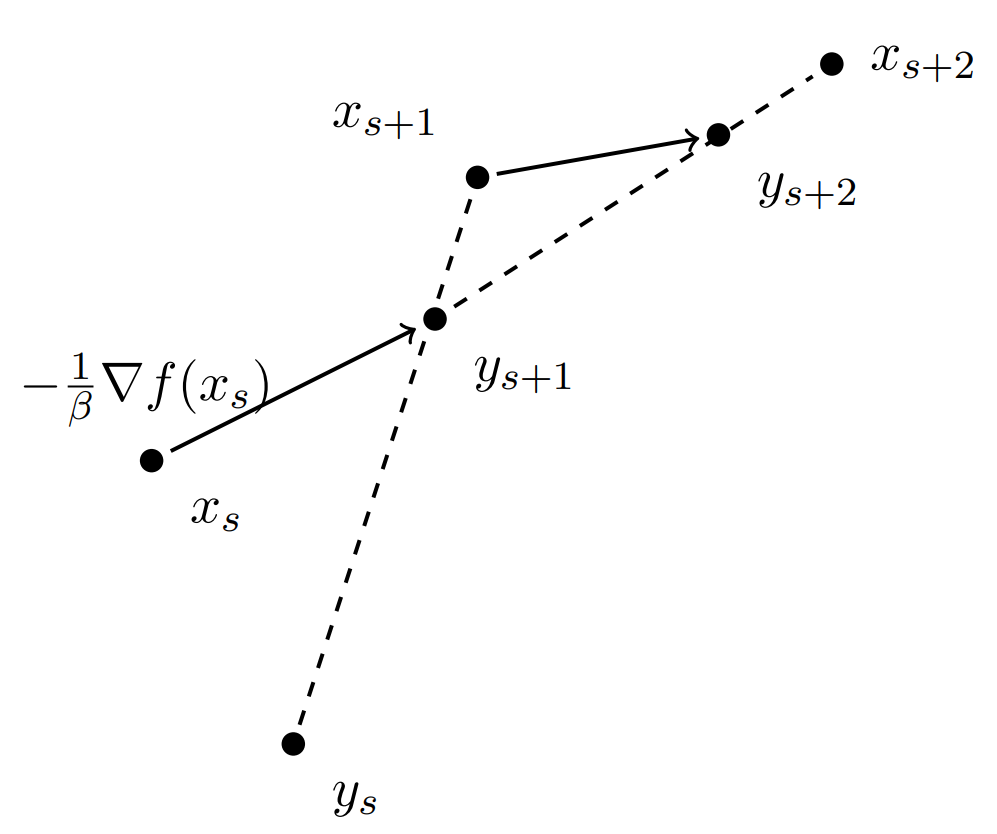
\includegraphics[width=0.35\textwidth]{./figures/fig_agd.png}
    
    \caption{Illustration of Nesterov’s accelerated gradient descent}
    \label{fig:figures}
    \end{figure}
    \begin{itemize}
        \item The idea of momentum is to include a term that capture some aspect of where 
        
        I was before, that is, the direction that I was moving in.
    \end{itemize}
\end{frame}

\begin{frame}\frametitle{ Nesterov’s Acceleration: $\beta$-smooth and $\alpha$-strongly convex functions}
\begin{spacing}{0.8}
\textbf{Nesterov's accelerated gradient descent can be described as follow:}
\begin{align*}
    x_1 &= y_1 \text{, iterate the following equations for }t\geq 1\\
    y_{t+1} &= x_t - {1 \over \beta} \nabla{f(x_t)} \\
    x_{t+1} &= {\left(1+{\sqrt{\kappa}-1 \over \sqrt{\kappa}+1}\right)}y_{t+1}-{\left({\sqrt{\kappa}-1 \over \sqrt{\kappa}+1}\right)}y_{t} \\
\end{align*}
\end{spacing}
\textbf{Theorem} {\it Let $f$ be $\alpha$-strongly convex and $\beta$-smooth, then Nesterov's accelerated gradient descent satisfies}

$$f(y_t)-f(x^*) \leq {\alpha+\beta \over 2}||x_1-x^*||^2 exp{\left(-{{t-1} \over \sqrt{\kappa}}\right)}$$
\end{frame}

\begin{frame}
\frametitle{ Nesterov’s Acceleration: $\beta$-smooth and $\alpha$-strongly convex functions}
    \begin{figure}[h]
    \centering
    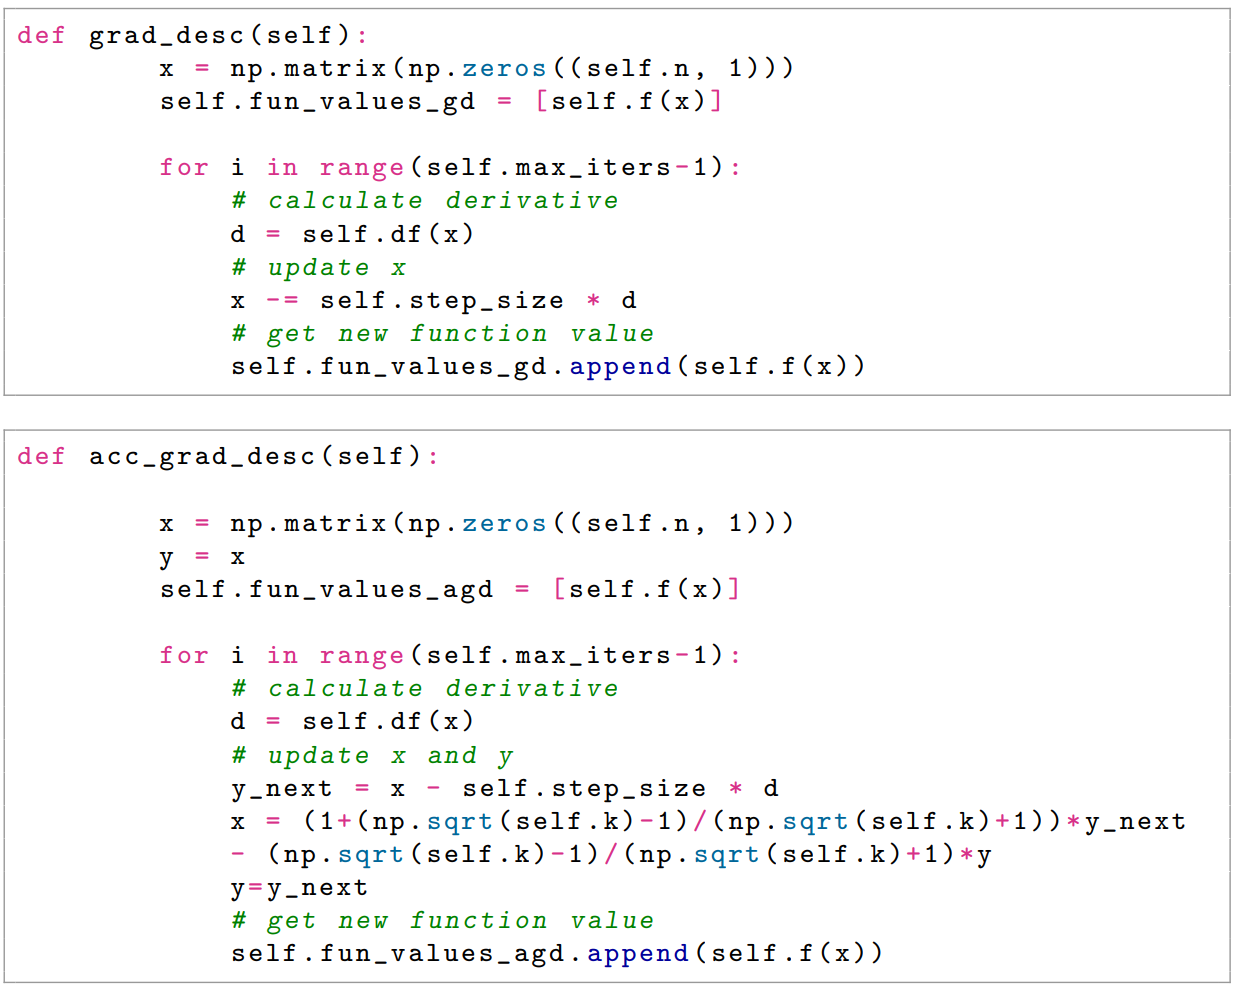
\includegraphics[width=0.7\textwidth]{./figures/fig_code.png}
    \end{figure}
\end{frame}

\begin{frame}
\frametitle{ Nesterov’s Acceleration: $\beta$-smooth and $\alpha$-strongly convex functions}
    \begin{figure}[h!]
    \centering
    \begin{subfigure}{0.49\textwidth}
        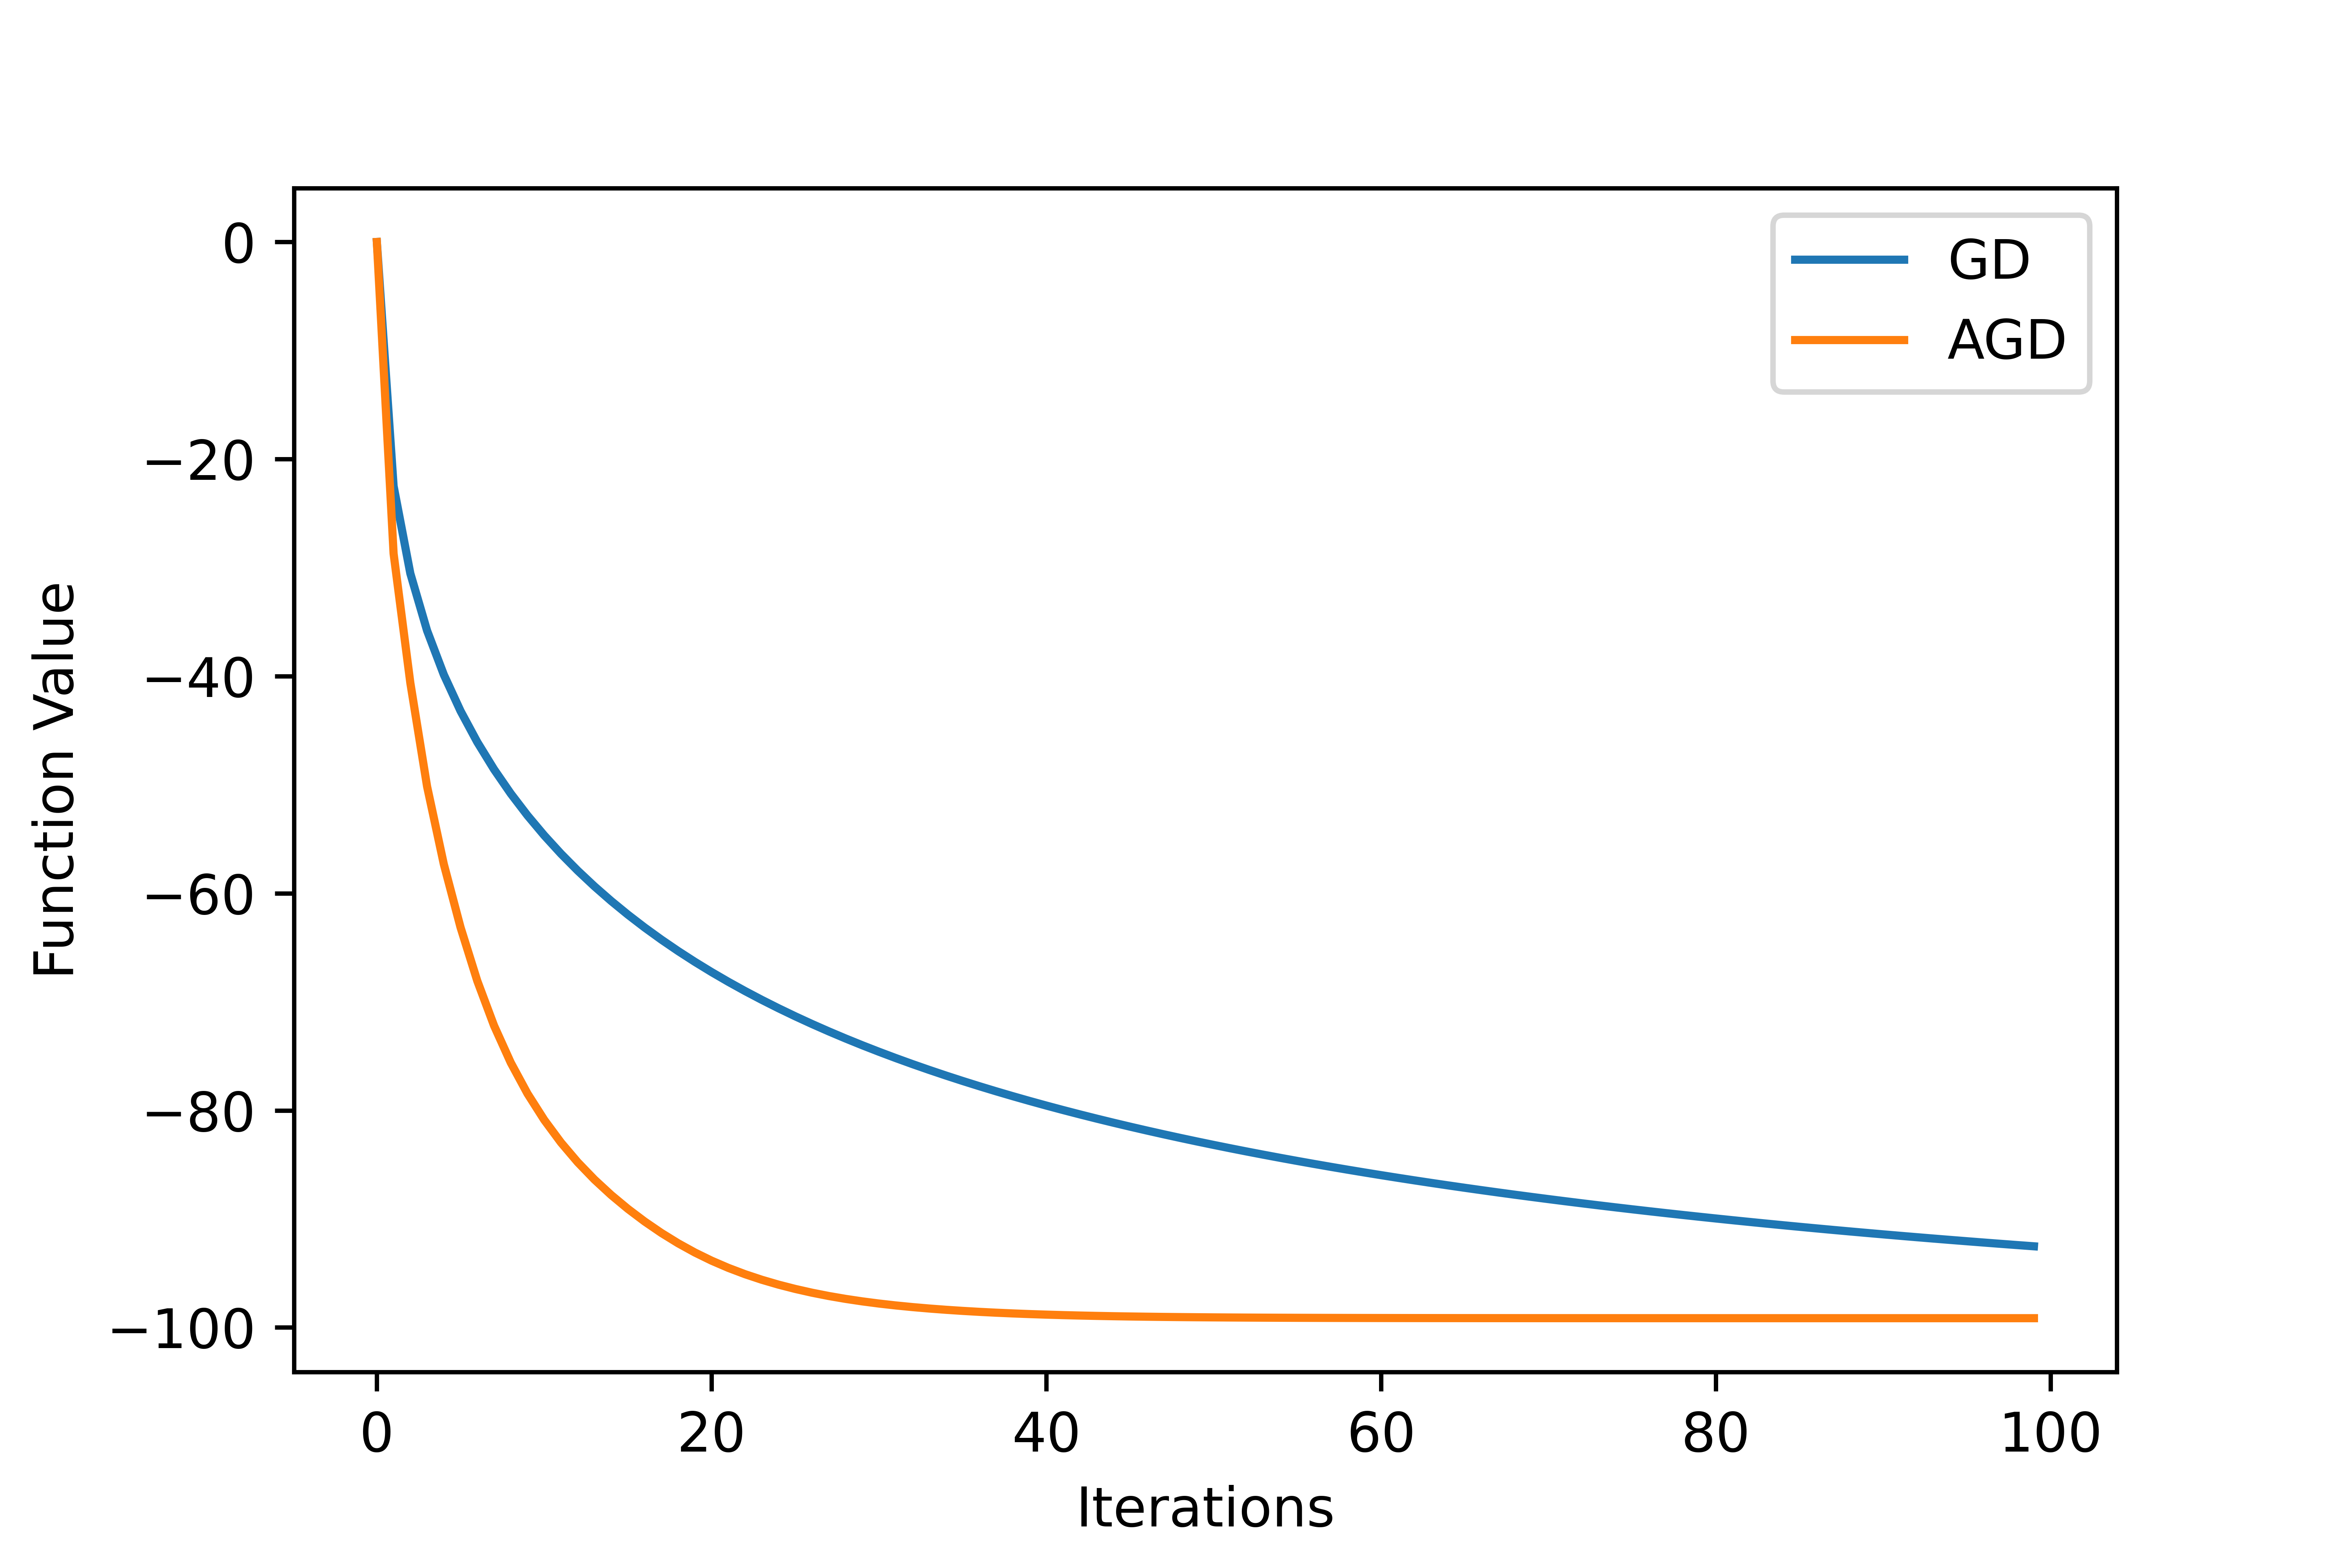
\includegraphics[width=\textwidth]{./figures/fig_r1.png}
        \caption{$\eta = 1$}
        \label{fig:first}
    \end{subfigure}
    \hfill
    \begin{subfigure}{0.49\textwidth}
        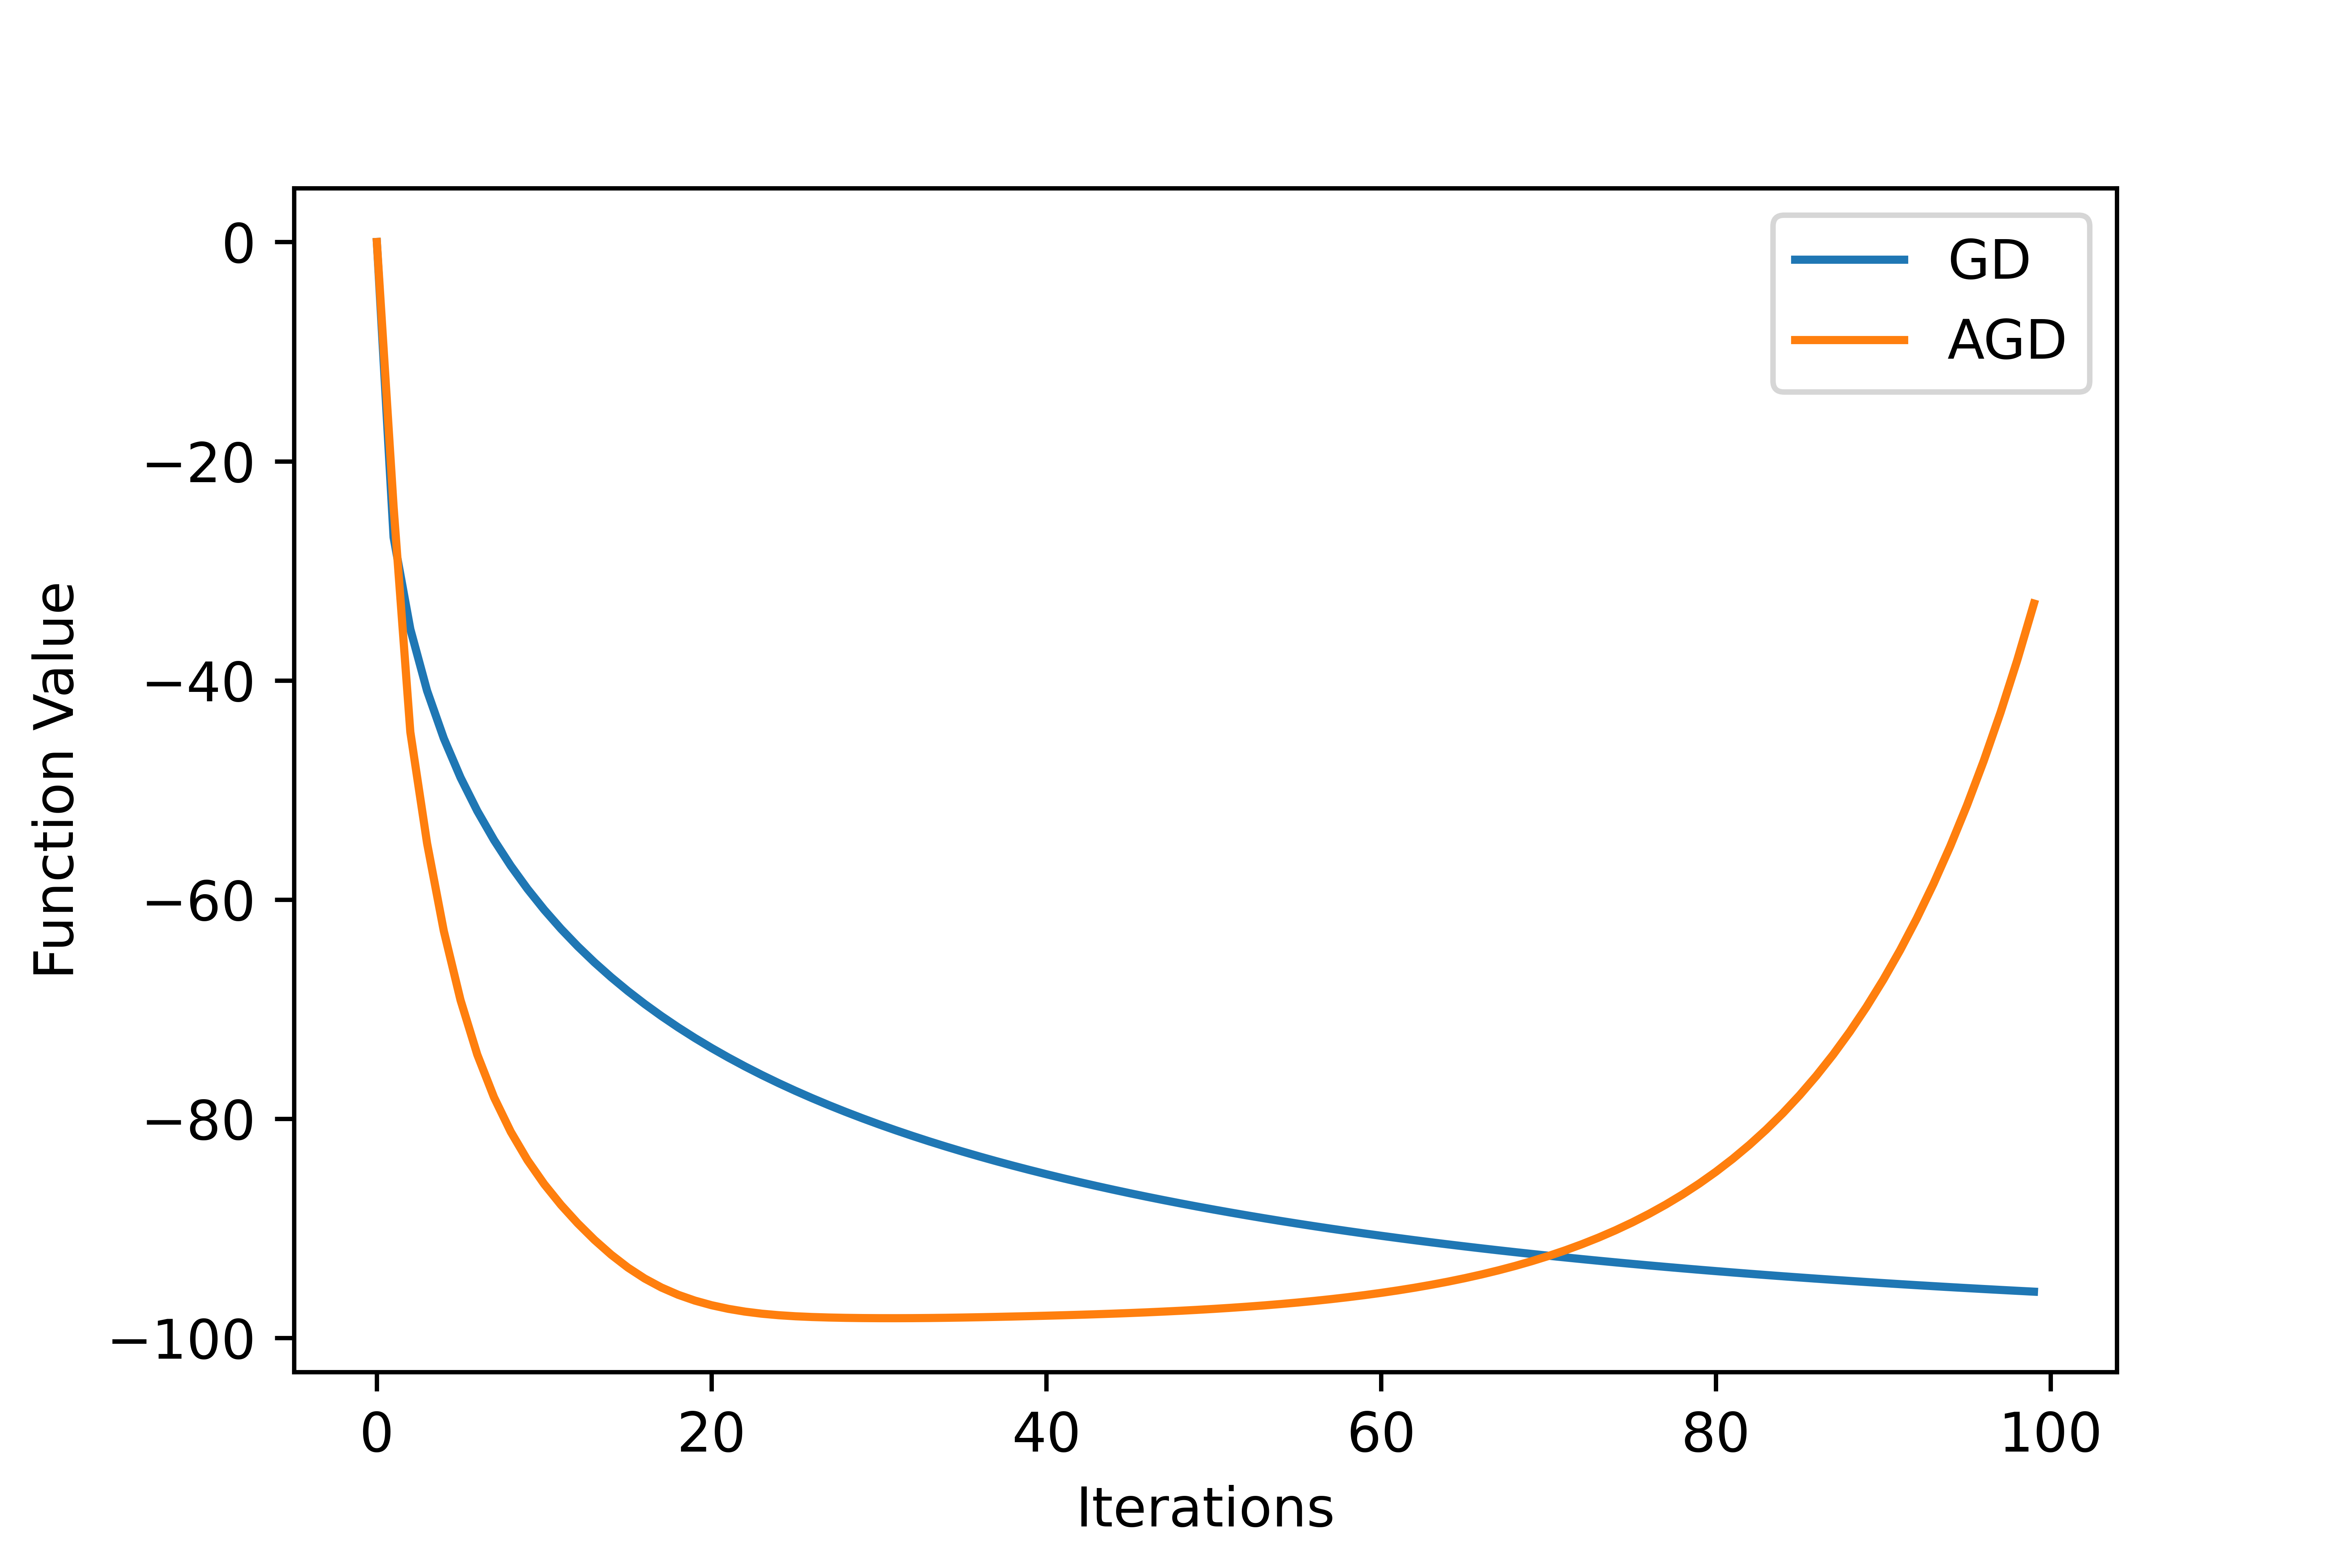
\includegraphics[width=\textwidth]{./figures/fig_r2.png}
        \caption{$\eta = 1.5$}
        \label{fig:second}
    \end{subfigure}
    \caption{Convergence rate of algorithms at different step size}
    \label{fig:figures}    
    \end{figure}

    \begin{itemize}
        \item Lower bounds for smooth,convex optimization are matched by AGD method

        \item Choose the coefficients carefully
    \end{itemize}
\end{frame}

\begin{frame}\frametitle{ Nesterov’s Acceleration: $\beta$-smooth and convex functions}
\begin{spacing}{0.5}
    

\textbf{Nesterov's accelerated gradient descent can be described as follow:}
\begin{align*}
    \lambda_0 &=0, \lambda_t = {1+\sqrt{1+4 {\lambda^2_{t-1}}} \over 2}, \gamma_t={1-\lambda_t \over \lambda_{t+1}} \leq 0\\
    x_1 &= y_1 \\
    y_{t+1} &= x_t - {1 \over \beta} \nabla{f(x_t)} \\
    x_{t+1} &= {\left(1-\gamma_t \right)}y_{t+1}+{{\gamma_t}}y_{t} \\
\end{align*}

\textbf{Theorem} {\it Let $f$ be a convex and $\beta$-smooth, then Nesterov's accelerated gradient descent satisfies}
\end{spacing}
$$f(y_t)-f(x^*) \leq {2\beta ||x_1-x^*||^2 \over t^2}$$
\end{frame}
    

\begin{frame}\frametitle{ Nesterov’s Acceleration: $\beta$-smooth and convex functions}

\textbf{Notation}

\begin{itemize}
    \item Gradient step: $x^{+}$ = $x$ - ${\eta}$${\nabla}$$f(x_t)$ , ${\eta}$=${1 \over \beta}$
    \item Momentum term: $d_t$ = $\gamma_t{\left(x_t - x_{t-1}\right)}$ , $\gamma_t$ is a parameter we choose
    \item Gradient descent algorithm: $x_{t+1}$ = $(x_t)^+$
    \item Nesterov's acceleration: $x_{t+1}$ = $(x_t + d_t)^+$ = $x_t+d_t$ - $\eta \nabla f(x_t+d_t)$
    \item $\delta_t = f(x_t) - f(x^*) \geq 0$  ,  $g_t = -{1 \over \beta}\nabla f(x_t+d_t)$
\end{itemize}

\setstretch{1.7}
\begin{lemma}

(a) $f(y) \leq f(x) + \langle\ \nabla f(x), x-y\rangle$ 

(b) $f(y) \leq f(x) + \langle\ \nabla f(x), x-y\rangle + {\beta \over 2}{||y-x||}^2$
$\rightarrow$ $f(x^+) - f(x) \leq - {1\over {2\beta}} ||\nabla f(x)||^2$ 

(c) $\delta_{t+1} - \delta_{t} \leq -{\beta \over 2}{\left(||g_t||^2 + 2g_t^Td_t\right)}$

(d) $\delta_{t+1} \leq -{\beta \over 2}{\left(||g_t||^2 + 2g_t^T\left(x_t+d_t-x^*\right)\right)}$

\end{lemma}

\end{frame}

\begin{frame}\frametitle{ Nesterov’s Acceleration: $\beta$-smooth and convex functions}
% \setstretch{1.5}
$$\delta_{t+1} - \delta_{t} \leq -{\beta \over 2}{\left(||g_t||^2 + 2g_t^Td_t\right)}$$
\begin{proof}

\begin{align*}
\delta_{t+1} - \delta_{t} &\leq -{\beta \over 2}{\left(||g_t||^2 + 2g_t^Td_t\right)} \\
&=  -{\beta \over 2}{\left({1 \over \beta^2}{||\nabla f(x_t+d_t)||}^2 -{2 \over \beta}\nabla f(x_t+d_t)^Td_t\right)} \\
&= -{1 \over 2\beta}||\nabla f(x_t+d_t)||^2+\nabla f(x_t+d_t)^Td_t \\
&\geq f \left(x_t+d_t-\eta \nabla f(x_t+d_t)\right) -f(x_t+d_t)+f(x_t+d_t) -f(x_t) (\because{b,a}) \\
&=\text{LHS}\\
\end{align*}

\end{proof}

\end{frame}

\begin{frame}\frametitle{ Nesterov’s Acceleration: $\beta$-smooth and convex functions}
% \setstretch{1.5}
$$\delta_{t+1} - \delta_{t} \leq -{\beta \over 2}{\left(||g_t||^2 + 2g_t^Td_t\right)}$$
\begin{proof}
 $$\text{(b) }f(x^+) - f(x) \leq - {1\over {2\beta}} ||\nabla f(x)||^2$$ 
\begin{align*}
  f \left(x_t+d_t-\eta \nabla f(x_t+d_t)\right) -f(x_t+d_t) &\leq -{1 \over 2\beta}||\nabla f(x_t+d_t)||^2  \\
\end{align*}

\begin{spacing}{0.05}
\end{spacing}

$$\text{(a) }f(y) \leq f(x) + \langle\ \nabla f(x), x-y\rangle = f(x)-\langle\ \nabla f(y), x-y\rangle$$ 
\begin{align*}
  f(x_t+d_t) -f(x_t) &\leq \nabla f(x_t+d_t)^Td_t  \\
\end{align*}

\end{proof}

\end{frame}


\begin{frame}\frametitle{ Nesterov’s Acceleration: $\beta$-smooth and convex functions}
% \setstretch{1.5}
$$\delta_{t+1} \leq -{\beta \over 2}{\left(||g_t||^2 + 2g_t^T\left(x_t+d_t-x^*\right)\right)}$$
\begin{proof}

\begin{align*}
\delta_{t+1}  &\leq -{\beta \over 2}{\left(||g_t||^2 + 2g_t^T\left(x_t+d_t-x^*\right)\right)} \\
&=  -{\beta \over 2}{\left({1 \over \beta^2}{||\nabla f(x_t+d_t)||}^2 -{2 \over \beta}\nabla f(x_t+d_t)^T\left(x_t+d_t-x^*\right)\right)} \\
&= -{1 \over 2\beta}||\nabla f(x_t+d_t)||^2+\nabla f(x_t+d_t)^T\left(x_t+d_t-x^*\right) \\
&\geq f \left(x_t+d_t\right) -f(x^*)+f(x_t) -f(x_t+d_t) (\because{b,a}) \\
&=\text{LHS}\\
\end{align*}

\end{proof}

\end{frame}

\begin{frame}\frametitle{ Nesterov’s Acceleration: $\beta$-smooth and convex functions}
% \setstretch{1.5}
$$\delta_{t+1} \leq -{\beta \over 2}{\left(||g_t||^2 + 2g_t^T\left(x_t+d_t-x^*\right)\right)}$$
\begin{proof}
$$\text{(b) }f(x^+) - f(x) \leq - {1\over {2\beta}} ||\nabla f(x)||^2 $$

$$f(x_t) -f(x_t+d_t)  \leq -{1 \over 2\beta}||\nabla f(x_t+d_t)||^2 $$

$$\text{(a) }f(y) \leq f(x) + \langle\ \nabla f(x), x-y\rangle = f(x)-\langle\ \nabla f(y), x-y\rangle$$

$$f \left(x_t+d_t\right) -f(x^*) \leq \nabla f(x_t+d_t)^T\left(x_t+d_t-x^*\right)$$


\end{proof}

\end{frame}


% \begin{frame}\frametitle{ Nesterov’s Acceleration: $\beta$-smooth and convex functions}

% \begin{proof}

% $(\lambda_t - 1)(\delta_{t+1} - \delta_{t}) + (\delta_{t+1}) \leq -{\beta \over 2}\left[{1 \over \lambda_t}\left(||x_t+\lambda_t d_t-x^*+\lambda_t g_t||^2-||x_t+\lambda_t d_t - x^*||^2\right)\right]$

% we would like for the RHS to be telescoping. 

% we want, $x_t+\lambda_t d_t - x^*+\lambda_t g_t$ = $x_{t+1}+\lambda_{t+1}d_{t+1}-x^*$

% recall : $d_{t+1} = \gamma_{t+1}(d_t+g_t)$

% \begin{align*}
% x_t+\lambda_t d_t - x^*+\lambda_t g_t &= x_{t+1}+\lambda_{t+1}d_{t+1}-x^*\\
% &=x_t+d_t+g_t+\lambda_{t+1}\gamma_{t+1}(d_t+g_t)-x^*
% \end{align*}

% if $\lambda_t(d_t+g_t) = (\lambda_{t+1}\gamma_{t+1}+1)(d_t+g_t)$ , then we can get what we want.

% $\gamma_t$ is a parameter that I'm able to choose. so I'm going to choose $\gamma_{t+1}$,$\gamma_t$ to make this telescope.


% \end{proof}

% \end{frame}

\begin{frame}\frametitle{ Nesterov’s Acceleration: $\beta$-smooth and convex functions}
\begin{spacing}{0.5}   

$$f(y_t)-f(x^*) \leq {2\beta ||x_1-x^*||^2 \over t^2}$$
\end{spacing}
\setstretch{1.2}
\begin{proof}



$(\lambda_t - 1)(\delta_{t+1} - \delta_{t}) + (\delta_{t+1}) \leq -{\beta \over 2}\left[{1 \over \lambda_t}\left(||x_t+\lambda_t d_t-x^*+\lambda_t g_t||^2-||x_t+\lambda_t d_t - x^*||^2\right)\right]$

\begin{center}
    we would like for the RHS to be telescoping. so we want , 

    $x_t+\lambda_t d_t - x^*+\lambda_t g_t$ = $x_{t+1}+\lambda_{t+1}d_{t+1}-x^*$

    recall : $x_{t+1}=x_t+d_t+g_t$, $d_{t+1} = \gamma_{t+1}(d_t+g_t)$
\end{center}

\begin{spacing}{0.5}
\begin{align*}
x_t+\lambda_t d_t - x^*+\lambda_t g_t &= x_{t+1}+\lambda_{t+1}d_{t+1}-x^*\\
&=x_t+d_t+g_t+\lambda_{t+1}\gamma_{t+1}(d_t+g_t)-x^*\\
\lambda_t(d_t+g_t)+x_t-x^* &= (\lambda_{t+1}\gamma_{t+1}+1)(d_t+g_t)+x_t-x^*
\end{align*}
\end{spacing}


\end{proof}

\end{frame}

\begin{frame}\frametitle{ Nesterov’s Acceleration: $\beta$-smooth and convex functions}
\setstretch{1.3}
$$f(y_t)-f(x^*) \leq {2\beta ||x_1-x^*||^2 \over t^2}$$

\begin{proof}


$(\lambda_t - 1)(\delta_{t+1} - \delta_{t}) + (\delta_{t+1}) \leq -{\beta \over 2}\left[{1 \over \lambda_t}\left(||x_t+\lambda_t d_t-x^*+\lambda_t g_t||^2-||x_t+\lambda_t d_t - x^*||^2\right)\right]$

$$\lambda_t(d_t+g_t)+x_t-x^* = (\lambda_{t+1}\gamma_{t+1}+1)(d_t+g_t)+x_t-x^*$$



if $\lambda_t(d_t+g_t) = (\lambda_{t+1}\gamma_{t+1}+1)(d_t+g_t)$ , then we can get what we want.

$\gamma_t$ is a parameter that I'm able to choose. so I'm going to choose $\gamma_{t+1}$,$\gamma_t$ to make this telescope.


\end{proof}

\end{frame}

% \begin{frame}\frametitle{ Nesterov’s Acceleration: $\beta$-smooth and convex functions}
% $$f(y_t)-f(x^*) \leq {2\beta ||x_1-x^*||^2 \over t^2}$$
% \begin{proof}


% ${2 \over \beta}u_{t+1}$ $\coloneqq ||x_t+\lambda_t d_t-x^*+\lambda_t g_t||^2$, 

% ${2 \over \beta}u_t$ $\coloneqq ||x_t+\lambda_t d_t - x^*||^2$

% multiplying by $\lambda_t$ and remember $\lambda_t$ is also a free parameter. $\gamma_t$ is a function of $\lambda_t$ that still allow me to pick,

% $\lambda_t^2(\delta_{t+1}) - (\lambda_t^2-\lambda_t)\delta_t$ $\leq u_t - u_{t+1}$

% we're going to pick $\lambda_t$ to make this telescope. that is It holds $\lambda_t^2 - \lambda_t=\lambda_{t-1}^2$ : $\lambda_t$ $\approx t$ will satisfy this, specifically: $\lambda_t = {-1\pm\sqrt{1+4\lambda_{t-1}^2} \over 2}$ 

% sum both sides for T iterations:

% $\lambda_T^2\delta_{T+1}-\lambda_0 \delta_1 \leq u_0 - u_T \leq u_0$ 
%  $\Rightarrow{\delta_{T+1}\leq {constant \over \lambda_T^2}}$

%  $\Rightarrow f(x_t)-f(x^*) \leq {constant\over T^2}$
% \end{proof}
% \end{frame}

\begin{frame}\frametitle{ Nesterov’s Acceleration: $\beta$-smooth and convex functions}
$$f(y_t)-f(x^*) \leq {2\beta ||x_1-x^*||^2 \over t^2}$$
\setstretch{1.5}
\begin{proof}
$(\lambda_t - 1)(\delta_{t+1} - \delta_{t}) + (\delta_{t+1}) \leq -{\beta \over 2}\left[{1 \over \lambda_t}\left(||x_t+\lambda_t d_t-x^*+\lambda_t g_t||^2-||x_t+\lambda_t d_t - x^*||^2\right)\right]$

\begin{center}
    

${2 \over \beta}u_{t+1}$ $\coloneqq ||x_t+\lambda_t d_t-x^*+\lambda_t g_t||^2$, ${2 \over \beta}u_t$ $\coloneqq ||x_t+\lambda_t d_t - x^*||^2$



$\lambda_t^2(\delta_{t+1}) - (\lambda_t^2-\lambda_t)\delta_t$ $\leq u_t - u_{t+1} (\because{\text{multiplying by } \lambda_t})$

\end{center}
 $\lambda_t$ is also a free parameter.$\gamma_t$ is a function of $\lambda_t$ that still allow me to pick.
\end{proof}
\end{frame}

\begin{frame}\frametitle{ Nesterov’s Acceleration: $\beta$-smooth and convex functions}
\begin{spacing}{0.5}
\end{spacing}
$$f(y_t)-f(x^*) \leq {2\beta ||x_1-x^*||^2 \over t^2}$$
\begin{proof}

$$\lambda_t^2(\delta_{t+1}) - (\lambda_t^2-\lambda_t)\delta_t \leq u_t - u_{t+1}$$

we're going to pick $\lambda_t$ to make this telescope. that is It holds
\begin{center}
    

$\lambda_t^2 - \lambda_t=\lambda_{t-1}^2$  ,so $\lambda_t = {-1\pm\sqrt{1+4\lambda_{t-1}^2} \over 2}$ $\approx t$ 
\begin{spacing}{2}
\end{spacing}
sum both sides for T iterations:
\begin{spacing}{0.005}
\end{spacing}
\begin{align*}
\lambda_T^2\delta_{T+1}-\lambda_0 \delta_1 \leq u_0 - u_T \leq u_0
&\Rightarrow{\delta_{T+1}\leq {constant \over \lambda_T^2}}\\
&\Rightarrow f(x_t)-f(x^*) \leq {constant\over T^2}
 \end{align*}

 \end{center}
\end{proof}
\end{frame}


\nocite{caramanis2020opt,
        bubeck2015convex}
\begin{frame}[t, allowframebreaks]{References}
    \printbibliography
    % NL: I think we should clean up `reference.bib`; it looks unncessarily complicated.
\end{frame}